%%%%%%%%%%%%%%%%%%%%%%%%%%%%%%%%%%%%%%%%%%%%%%%%%%%%%%%%%%%%%%%%%%%%%%%%%
% ARTICLE ABOUT FATE OF SYNONYMOUS MUTATIONS IN HIV
%%%%%%%%%%%%%%%%%%%%%%%%%%%%%%%%%%%%%%%%%%%%%%%%%%%%%%%%%%%%%%%%%%%%%%%%%
%\documentclass[pre, onecolumn, preprint]{revtex}
\documentclass[11pt]{article}
%%%%%%%%%%%%%%%%%%%%%%%%%%%%%%%%%%%%%%%%%%%%%%%%%%%%%%%%%%%%%%%%%%%%%%%%%
%%%%%%%%%%%%%%%%%%%%%%%%%%%%%%%%%%%%%%%%%%%%%%%%%%%%%%%%%%%%%%%%%%%%%%%%%
\usepackage[english]{babel}
\usepackage[utf8x]{inputenc}
\usepackage{amsmath,amsfonts,amssymb,eucal,eurosym,textcomp}
\usepackage{color}
\usepackage{graphicx}
\usepackage[numbers]{natbib}
\usepackage{lineno}
\linenumbers

%%%%%%%%%%%%%%%%%%%%%%%%%%%%%%%%%%%%%%%%%%%%%%%%%%%%%%%%%%%%%%%%%%%%%%%%%
\graphicspath{{./figures/}}
%%%%%%%%%%%%%%%%%%%%%%%%%%%%%%%%%%%%%%%%%%%%%%%%%%%%%%%%%%%%%%%%%%%%%%%%%
\newcommand{\comment}[1]{\textit{\textcolor{red}{#1}}}
\newcommand{\mut}{\mu}
\newcommand{\mfit}{\langle F\rangle}
\newcommand{\mexpfit}{\langle e^{F}\rangle}
\newcommand{\pfix}{P_{\mathrm{fix}}}
\newcommand{\ox}{r}
\newcommand{\co}{\rho}
\newcommand{\gt}{g}
\newcommand{\locus}{s}
\newcommand{\locuspm}{t}
\newcommand{\OO}{\mathcal{O}}
\newcommand{\FIG}[1]{Fig.~\ref{fig:#1}}
\newcommand{\FIGS}[2]{Figs.~\ref{fig:#1} and~\ref{fig:#2}}
\newcommand{\env}{\textit{env}}
\newcommand{\rev}{\textit{rev}}
\newcommand{\pol}{\textit{pol}}
\newcommand{\shankaregion}{C2-V5}
\newcommand{\PCApat}{1}
\newcommand{\syndiv}{2}
\newcommand{\timedependence}{3}
\newcommand{\withinepi}{4}
\newcommand{\marginals}{5}
%%%%%%%%%%%%%%%%%%%%%%%%%%%%%%%%%%%%%%%%%%%%%%%%%%%%%%%%%%%%%%%%%%%%%%%%%
\newcommand{\Author}{Fabio~Zanini and Richard~A.~Neher}
\newcommand{\Title}{Quantifying selection against synonymous mutations in HIV-1 \env{} evolution}
\newcommand{\Affiliation}{Max Planck Institute for Developmental Biology, 72076 T\"ubingen, Germany}
\newcommand{\Keywords}{{HIV}, {synonymous}, {population genetics}}
%%%%%%%%%%%%%%%%%%%%%%%%%%%%%%%%%%%%%%%%%%%%%%%%%%%%%%%%%%%%%%%%%%%%%%%%%
\usepackage{hyperref}
\hypersetup{colorlinks,linkcolor=red,citecolor=blue, pdfauthor={\Author}, pdftitle={\Title}, pdfkeywords={\Keywords}}
%%%%%%%%%%%%%%%%%%%%%%%%%%%%%%%%%%%%%%%%%%%%%%%%%%%%%%%%%%%%%%%%%%%%%%%%%
\linespread{1.5}
\begin{document}
\title{\Title}
\author{\Author\\ \Affiliation}
\date{\today}
%%%%%%%%%%%%%%%%%%%%%%%%%%%%%%%%%%%%%%%%%%%%%%%%%%%%%%%%%%%%%%%%%%%%%%%%%
\maketitle

\newpage
\section*{Abstract}
\noindent
Intrapatient HIV-1 evolution is driven by the adaptive immune system
resulting in rapid change of HIV-1 proteins. When cytotoxic CD8${}^+$
T-cells or neutralizing antibodies target a new epitope, the virus often
escapes via nonsynonymous mutations that impair recognition. Synonymous
mutations do not affect this interplay and are often assumed to be
neutral. We test this assumption by tracking synonymous mutations in
longitudinal intrapatient data from the \shankaregion{} part of the
\env{} gene. We find that most synonymous variants are lost even though
they often reach high frequencies in the viral population, suggesting a
cost to the virus. Using published data from SHAPE assays, we find that
synonymous mutations that disrupt base pairs in RNA stems flanking the
variable loops of gp120 are more likely to be lost than other synonymous
changes: these RNA hairpins might be important for HIV-1.  Computational
modeling indicates that, to be consistent with the data, a large fraction
of synonymous mutations in this genomic region needs to be deleterious,
with a cost of the order of $0.002$ per day. This weak selection against synonymous
substitutions does not result in a strong pattern of conservation in
cross sectional data, but slows down the rate of evolution
considerably. Our findings are consistent with the notion that large
scale patterns of RNA structure are functionally relevant, while the
precise base pairing pattern is not.
%%%%%%%%%%%%%%%%%%%%%%%%%%%%%%%%%%%%%%%%%%%%%%%%%%%%%%%%%%%%%%%%%%%%%%%%%
\section*{Introduction}
%%%%%%%%%%%%%%%%%%%%%%%%%%%%%%%%%%%%%%%%%%%%%%%%%%%%%%%%%%%%%%%%%%%%%%%%%
HIV-1 evolves rapidly within a single host during the course of the infection.
This evolution is driven by strong selection imposed by the host immune system
via cytotoxic CD8${}^+$ T-cells (CTLs) and neutralizing antibodies
(nAbs)~\citep{rambaut_causes_2004} and facilitated by HIV-1's high mutation rate
~\citep{mansky_lower_1995,abram_nature_2010}. Escape mutations
in epitopes targeted by CTLs are typically observed during early infection and spread
rapidly through the population~\citep{mcmichael_immune_2009}. During chronic
infection, the most rapidly evolving parts of the HIV-1 genome are the variable
loops V1-V5 in the envelope protein gp120 (V loops), which change to avoid recognition by
nAbs. Escape mutations in \env{}, the gene encoding gp120, spread through the
viral population within a few months.
Consistent with this time scale, it is found that serum from a particular time
typically neutralizes autologous virus extracted more than 3-6 months earlier but not contemporary
virus \citep{richman_rapid_2003}.

Escape mutations are selected because they change the amino acid sequence of
viral proteins in a way that reduces antibody binding or epitope presentation.
Conversely, synonymous mutations do not modify the viral proteins and are
commonly used as approximately neutral markers in studies of viral evolution,
i.e., as a negative control for detecting selected
sites \citep{Bhatt:2011p43255,Hurst:2002p32608,Chen:2004p22606}. In addition to
maintaining protein function and avoiding the adaptive immune recognition,
however, the HIV-1 genome has to ensure efficient processing and translation,
nuclear export, and packaging into the viral capsid: all these processes operate
at the RNA level and are sensitive to synonymous changes. Several
important RNA secondary structures have been characterized in detail, including the HIV-1
\rev{} response element (RRE) in \env{} which enhances nuclear export of full length
or partially spliced viral transcripts via a complex hairpin RNA structure
\citep{fernandes_hiv-1_2012}. In fact, the HIV-1 genome is full of RNA
structures \citep{watts_architecture_2009} with no or unknown
function. However, large scale modification of secondary structures
can result in substantial reduction of the replication capacity
\citep{keating_rich_2009} and the propensity of forming RNA stems
anticorrelates with the rate of evolution
\citep{forsdyke_reciprocal_1995,snoeck_mapping_2011}. 
These poorly characterized RNA structures are conserved to varying degree between HIV-1 and
SIV: corresponding regions tend to be part
of similar structural elements, but individual base pairings are very
rarely conserved \citep{pollom_comparison_2013}. 

In this paper, we characterize the dynamics of synonymous mutations in \env{}
and show that, in the region of the V loops, a large fraction of these mutations
is deleterious. Despite their fitness cost, deleterious synonymous variants
rise in frequency in the viral population via genetic hitchhiking due to limited
recombination in HIV-1 populations~\citep{neher_recombination_2010,
batorsky_estimate_2011}. We show a strong correlation between the fate of a
synonymous variant and the surrounding RNA structure. We then compare our
observations to computational models and obtain estimates for the effect of
synonymous mutations on viral fitness.

%%%%%%%%%%%%%%%%%%%%%%%%%%%%%%%%%%%%%%%%%%%%%%%%%%%%%%%%%%%%%%%%%%%%%%%%%
\section*{Materials \& Methods}
%%%%%%%%%%%%%%%%%%%%%%%%%%%%%%%%%%%%%%%%%%%%%%%%%%%%%%%%%%%%%%%%%%%%%%%%%
\subsection*{Sequence data collection}
%%%%%%%%%%%%%%%%%%%%%%%%%%%%%%%%%%%%%%%%%%%%%%%%%%%%%%%%%%%%%%%%%%%%%%%%%
Longitudinal intrapatient viral RNA sequences were collected from published
studies \citep{shankarappa_consistent_1999, liu_selection_2006,
bunnik_autologous_2008} and downloaded from the Los Alamos National Laboratory
(LANL) HIV sequence database~\citep{LANL2012}. Some patients
show substantial population structure and were excluded (see
Fig.~S\PCApat); a total of 11 patients with 4-23 time points each and
approximately 10 sequences per time point were analyzed. The time intervals
between two consecutive sequences ranged from 1 to 34 months, most of them
between 6 and 10 months.

%%%%%%%%%%%%%%%%%%%%%%%%%%%%%%%%%%%%%%%%%%%%%%%%%%%%%%%%%%%%%%%%%%%%%%%%%
\subsection*{Sequence analysis}
%%%%%%%%%%%%%%%%%%%%%%%%%%%%%%%%%%%%%%%%%%%%%%%%%%%%%%%%%%%%%%%%%%%%%%%%%
The sequences were translated and the resulting amino acid sequences aligned
using Muscle~\citep{edgar_muscle:_2004} to each other and the NL4-3 reference
sequence separately for each patient. Within each patient, the consensus
nucleotide sequence at the first time point was used to classify alleles as
``ancestral'' or ``derived'' at all sites. Sites that include large
frequencies of gaps were excluded from the analysis to avoid artifactual
substitutions due to alignment errors. Allele frequencies at different time
points were extracted from the multiple sequence alignment.

A mutation was considered synonymous if it did not change the amino acid
corresponding to the codon, and if the rest of the codon was in the ancestral
state. Codons with more than one mutation were discarded. Slightly different
criteria for synonymous/nonsynonymous discrimination yielded similar results.

%%%%%%%%%%%%%%%%%%%%%%%%%%%%%%%%%%%%%%%%%%%%%%%%%%%%%%%%%%%%%%%%%%%%%%%%%
\subsection*{Fixation probability and secondary structure}
%%%%%%%%%%%%%%%%%%%%%%%%%%%%%%%%%%%%%%%%%%%%%%%%%%%%%%%%%%%%%%%%%%%%%%%%%
For the estimates of time to fixation/extinction, single nucleotide variants
(SNVs) were binned by
frequency and the time to first reaching either fixation or extinction was
stored. The fixation probability was determined as the long-time limit of the
resulting curves. Mutations that reached high frequency but neither fixed nor
were lost were classified as ``floating'' unless they first
reached high frequencies within 3 years of the last time point. In that case, it was assumed
they had not had sufficient time to fix and were discarded.

The SHAPE scores quantifying the degree of base pairing of individuals sites in
the HIV-1 genome were downloaded from the journal website
\citep{watts_architecture_2009}. Wherever possible, SHAPE reactivities were
assigned to sites in the multiple sequence alignments for each patient through
the alignment to the sequence of the NL4-3 virus used in
\citep{watts_architecture_2009}. Problematic assignments in indel-rich
regions were excluded from the analysis. The variable loops and flanking
regions were identified manually starting from the annotated reference HXB2
sequence from the LANL HIV database~\citep{LANL2012}. 

%%%%%%%%%%%%%%%%%%%%%%%%%%%%%%%%%%%%%%%%%%%%%%%%%%%%%%%%%%%%%%%%%%%%%%%%%
\subsection*{Computer simulations}
%%%%%%%%%%%%%%%%%%%%%%%%%%%%%%%%%%%%%%%%%%%%%%%%%%%%%%%%%%%%%%%%%%%%%%%%%
Computer simulations were performed using FFPopSim
\citep{zanini_ffpopsim:_2012}. Briefly, FFPopSim enables individual-based
simulations where each site in the genome is represented by one bit that can be
in one of two states. Outcrossing rates, crossover rates, mutation rates and
arbitrary fitness functions can be specified. While the best estimates
for the HIV generation time is roughly two days
\citep{perelson_hiv-1_1996, markowitz_novel_2003}, the generation time
has very little influence on the result and basically sets the unit of
time in which other parameters are measured. For simplicity, we use one
generation per day and have checked that the results obtained are
indistinguishable from simulations with a generation time of two days.

\subsubsection*{Parameters}
In order to simulate HIV, we have to specify several parameters that are
known to various degrees. The mutation rate has been measured using
exogenous LacZ constructs and the average nucleotide substitution rate is 
estimated to be $\mu\approx 2 \cdot 10^{-5}$ per generation \citep{mansky_lower_1995,
abram_nature_2010}. In our simulations, we vary the mutations rate
from $10^{-5} - 4\cdot 10^{-5}$ per day. Different virions within an
infected person can recombine their genome by coinfection of the same
cell, followed by template switching during reverse transcription. 
Template switching happens between around ten times per reverse
transcription \citep{levy_dynamics_2004}. The combined recombination rate of template
switching and coinfection has been estimated based on modeling to be around $\rho\approx
10^{-5}$ per nucleotide and day
\citep{neher_recombination_2010,batorsky_estimate_2011}, implying a
coinfection rate of a few percent or less, as has been recently
confirmed experimentally \citep{josefsson_single_2013}. We assume a
template switching rate of $10^{-3}$ per nucleotide and vary the
recombination rate between $5\cdot 10^{-6}- 5\cdot 10^{-5}$ by adjusting the
coinfection rate. The population size relevant to evolution in chronic
infection has been hotly debated. The number of cells infected by HIV-1
per day is on the order of $10^{7}$ \citep{perelson_hiv-1_1996}, but the
number of viruses contributing to the next generation might be
considerably smaller due to the burstiness of replication. 
Recent evidence points to a relevant population
size in excess of the inverse mutation rate
\citep{boltz_ultrasensitive_2012}. In fact, the evolutionary dynamics
depends only weakly on the actual value of the population size once the
product $N\mu$ is of order one or larger \citep{neher_genetic_2011}. We
simulate populations between $N=10^4$ and $5 \cdot 10^4$. Larger populations
become prohibitively costly to simulate.

Another crucial ingredient for our simulations is the fitness landscape,
i.e., the effects of mutations on fitness and possible interactions
between mutations. For simplicity, third positions of every codon were
deemed synonymous and assigned either a selection coefficient $0$ with
probability $\alpha$ or a deleterious effect $s_d$ with probability
$1-\alpha$. In our simulations, $\alpha$ varies from 0 to 0.75,
and $s_d$ between $2 \cdot 10^{-4}$ to $2\cdot 10^{-2}$ per day.
Mutations at the first and second positions were assigned deleterious 
fitness effects of $-0.01$ (simulations with a larger cost of $-0.1$ were also
performed and produced similar results). At 
rate $k_A$, a random locus in the genome is designated an epitope that can
escape by one or several mutations with exponentially distributed escape rates
with mean $\epsilon$. The rate of escape in chronic infection is
reported to be on the order of a few percent
\citep{Asquith:2006p28003,moore_limited_2009}, consistent with the
finding that virus is neutralized by serum from 3-6 month later
\citep{richman_rapid_2003}. We simulated escape rates between $2 \cdot
10^{-2.5}$ and $2 \cdot 10^{-1.5}$ per day. 
The rate $k_A$ at which new antibody challenges arise is more difficult to
quantify, but a substantial fraction of nonsynonymous substitutions in gp120 are
probably driven by escape. We simulate a range from $10^{-3.8}$ to $2\cdot 10^{-2}$ per day.

For the models with competition within epitopes, a complex epistatic fitness
landscape was designed such that each single mutant is sufficient for full
escape. Specifically, each mutation has an additive effect equal to the
escape rate, but interacts with all other escape mutations in the same
epitope with a negative effect of the same magnitude. 
Higher order terms were included to make sure that not
only double mutants, but all k-mutants with $k \geq 1$ had the same fitness (see
supplementary materials). To model recognition of escape variants by the
evolving immune system, the beneficial effect of an escape mutation was set
to its previous cost of $-0.01$ with a probability per generation proportional to
the frequency of the escape variant.

\subsubsection*{Sampling and analysis}
To obtain reasonable sampling of a particular parameter combination we
ran simulation for 6000 days and we repeated each run 100 times with
different seeds for the random number generator. Both full-length HIV-1
genomes and \env{}-only simulations were performed and yielded
comparable results. Populations were initialized with a homogeneous
founder population. After 30 generations of burn-in to create
genetic diversity, new epitopes were introduced at random with rate
$k_A$. The simulations were repeated 3000 times with a seven dimensional
Latin hypercube sampling scheme \citep{mckay_comparison_1979}, bounded by the ranges
given for each of these parameters above. For all parameter but the
fraction $\alpha$ of neutral sites,  parameters were sampled uniformly in
log-space. 

The areas below or above the neutral fixation probability (diagonal line) were
estimated from the binned fixation probabilities using linear interpolation
between the bin centers. The bins used were $[0.1, 0.2], [0.2, 0.4],
[0.4, 0.6]$, which is sufficiently precise for our purposes. Note that
we did not consider the frequency interval between 0.6 and 1, since very
few variants are observed in this window and its inclusion generates
more noise than signal.
 
%%%%%%%%%%%%%%%%%%%%%%%%%%%%%%%%%%%%%%%%%%%%%%%%%%%%%%%%%%%%%%%%%%%%%%%%%
\subsection*{Methods availability}
%%%%%%%%%%%%%%%%%%%%%%%%%%%%%%%%%%%%%%%%%%%%%%%%%%%%%%%%%%%%%%%%%%%%%%%%%
All analysis and computer simulation scripts, as well as the sequence alignments
used, are available for download at \url{http://git.tuebingen.mpg.de/synmut}.


%%%%%%%%%%%%%%%%%%%%%%%%%%%%%%%%%%%%%%%%%%%%%%%%%%%%%%%%%%%%%%%%%%%%%%%%%
\section*{Results}
%%%%%%%%%%%%%%%%%%%%%%%%%%%%%%%%%%%%%%%%%%%%%%%%%%%%%%%%%%%%%%%%%%%%%%%%%
Due to the large population size and the high mutation rate, every
possible single nucleotide variant (SNV) is produced multiple times per
day \citep{coffin_hiv_1995}. Some of these variants rise to high enough
frequency that they are observed in a sample of sequences. SNVs rise or fall in 
frequency because of three reasons: (i) their own effect on fitness and escape; (ii)
their association to genetic backgrounds; (iii) stochastic fluctuations
(genetic drift). We study the dynamics of sample frequencies, $\nu$, of SNVs,
i.e., the fraction $\nu$ of the sequences in a sample carrying
the variant. When an SNVs is present in all sequences 
at a certain time point, we say it has ``fixed''; when it is completely absent,
we say it was ``lost'' or is ``extinct''. 

Most positions are only transiently variable and variants will either fix or
will be lost -- at least in small samples. Given an SNV is at a certain
frequency $\nu$, the probability of fixation is higher for beneficial
SNVs than for neutral ones; in turn, neutral variants fix more frequently than
deleterious ones. The fixation probability of a
neutral SNV at frequency $\nu$ is the frequency itself, i.e.,
$\pfix(\nu) = \nu$, while it goes extinct with probability $1-\nu$. For
instance, if a neutral SNV is observed in half of the sequences, it will
fix with a probability of 50\% (see inset in figure
\ref{fig:aft}A). The fixation probability of neutral SNVs is
independent of most model assumptions and is only affected if neutral
SNVs are associated preferentially with either high or low fitness
virus.

\FIG{aft} shows the time course of the frequencies of all synonymous
SNVs (top) and nonsynonymous SNVs (bottom) observed in the
\shankaregion{} region of \env{} in a chronically HIV-1 infected patient (p10 from
\citet{shankarappa_consistent_1999}). Despite many synonymous SNVs
reaching high frequency, very few fix (Fig.~\ref{fig:aft}A); in
contrast, many nonsynonymous mutations fix
(Fig.~\ref{fig:aft}B). This observation seems at odds with
the assumption of neutrality.

%%%%%%%%%%%%%%%%%%%%%%%%%%%%%%%%%%%%%%%%%%%%%%%%%%%%%%%%%%%%%%%%%%%%%%%%%
\subsection*{Many synonymous SNVs in \shankaregion{} are deleterious}
%%%%%%%%%%%%%%%%%%%%%%%%%%%%%%%%%%%%%%%%%%%%%%%%%%%%%%%%%%%%%%%%%%%%%%%%%
We studied the dynamics and fate of synonymous variants more quantitatively by
analyzing data from seven patients from \citet{shankarappa_consistent_1999} and
\citet{liu_selection_2006} as well as three patients from
\citet{bunnik_autologous_2008} (patients with strong viral population structure
were not considered; see methods and Fig.~S\PCApat). The
former data set is restricted to the \shankaregion{} region of \env, while the
data from \citet{bunnik_autologous_2008} cover most of \env.  We considered all
SNVs in a frequency interval $[\nu_0-\delta\nu, \nu_0+\delta\nu]$ at some time
$t$, and calculated the fraction that are still observed at later times $t+\Delta
t$. Plotting this fraction against the time interval $\Delta t$, we see that
most synonymous SNVs segregate for roughly one year and are lost much more
frequently than expected under neutrality (Fig.~\ref{fig:fixp}A). The long-time
probability of fixation, $\pfix$, is shown as a function of the initial
frequency $\nu_0$ in Fig.~\ref{fig:fixp}B. The neutral expectation is
shown as a black dashed line. We found that $\pfix$ of synonymous
variants is far below the neutral expectation in \shankaregion{} (red line).
Outside of \shankaregion, using data from \citet{bunnik_autologous_2008} only,
we found no such reduction in $\pfix$ (green line). Restricted to the
\shankaregion{} region, the sequence samples from \citet{bunnik_autologous_2008}
are fully compatible with data from \citet{shankarappa_consistent_1999}
and show that synonymous mutations fix less often then expected under neutrality. The
nonsynonymous SNVs seem to follow more or less the neutral expectation (blue
line) -- a point to which we come back below.

When interpreting these results for the fixation probabilities, it is important
to note that we focused on SNVs that have already reached high frequencies. In
HIV-1 infection, most SNVs remain very rare throughout: they are not considered
here. Synonymous SNVs can reach high frequencies either through genetic
drift or genetic hitchhiking on escape variants (see below); very deleterious
variants will never reach high frequencies in the first place. Hence, our
analysis indicates that, among all synonymous SNVs that somehow reach high
frequencies, most of those in \shankaregion{} are deleterious, while
those in the rest of \env{} tend to be neutral.

%%%%%%%%%%%%%%%%%%%%%%%%%%%%%%%%%%%%%%%%%%%%%%%%%%%%%%%%%%%%%%%%%%%%%%%%%
\subsection*{Synonymous mutations in \shankaregion{} tend to disrupt RNA stems}
%%%%%%%%%%%%%%%%%%%%%%%%%%%%%%%%%%%%%%%%%%%%%%%%%%%%%%%%%%%%%%%%%%%%%%%%%
One possible explanation for a reduced fixation of synonymous variants in
\shankaregion{} is secondary structure in the viral RNA, the disruption of which
is deleterious to the virus \citep{forsdyke_reciprocal_1995,
snoeck_mapping_2011, sanjuan_interplay_2011}.

The propensity of nucleotides in the HIV-1 genome to form base pairs has been
measured using the SHAPE assay, a biochemical reaction preferentially altering
unpaired bases 
\citep{watts_architecture_2009}. The SHAPE assay has shown that the variable
regions V1-V5 tend to be unpaired, while the conserved regions between those
stretches form stems. We aligned the sequences from each patient to
the reference NL4-3 strain used in \citet{watts_architecture_2009} and assigned
SHAPE reactivities to most positions in the alignment. We then calculated the
distributions of SHAPE reactivities for synonymous SNVs that fixed or were
lost (only variants reaching frequencies above 15\%). As shown in
\FIG{SHAPE}A, the reactivities of fixed SNVs (red histogram) are systematically
larger than those of lost SNVs (blue) (Kolmogorov-Smirnov test on the cumulative
distribution, $p\approx 0.002$). In other words, SNVs that are likely to
break RNA helices are also more likely to revert and finally be lost from the
population, restoring the helix. Note that this analysis will be sensitive only
at positions where the base pairing pattern of NL4-3 agrees with that of each
patient's initial consensus sequence -- it is thus statistically conservative.
As a control, we also calculate the distribution of SHAPE reactivities for SNVs
that never reach high frequencies (green). This set is a mixture of neutral and
deleterious SNVs and, as expected, its distribution lies between those of
fixed and lost high-frequency variants.

To test the hypothesis that synonymous variants in \shankaregion{} are lost because they
break stems in the conserved stretches between the V loops, we considered
separately SNVs in V loops and their flanks. The greatest
depression in fixation probability is observed in the conserved stems, while the
V loops show little deviation from the neutral signature, see
\FIG{SHAPE}B. This is suggestive of important RNA helices in conserved
regions between the V loops.

In addition to RNA secondary structure, we have considered other possible
explanations for a fitness cost of some synonymous mutations, in particular
codon usage bias (CUB). HIV-1 is known to prefer A-rich codons over highly
expressed human codons \citep{jenkins_extent_2003, kuyl_biased_2012}. We
did not find any evidence for a contribution of average CUB to the ultimate
fate of synonymous SNVs; this is consistent with the observation that HIV-1 is not
adapting its codon usage to its human host cells at the macro-evolutionary level
\citep{kuyl_biased_2012}.


%%%%%%%%%%%%%%%%%%%%%%%%%%%%%%%%%%%%%%%%%%%%%%%%%%%%%%%%%%%%%%%%%%%%%%%%%
\subsection*{Deleterious SNVs can reach high frequency by hitchhiking}
%%%%%%%%%%%%%%%%%%%%%%%%%%%%%%%%%%%%%%%%%%%%%%%%%%%%%%%%%%%%%%%%%%%%%%%%%
While the observation that some synonymous variants are deleterious is not
unexpected, it seems odd that we observe them at high population
frequency and that the fixation probability is reduced only in parts of the
genome (in \shankaregion{} but not in the rest of \env{}; compare the red
and green lines in \FIG{fixp}B).
The region \shankaregion{} undergoes frequent adaptive changes to evade
recognition by neutralizing antibodies \cite{williamson_adaptation_2003,wei_antibody_2003,
richman_rapid_2003}. Due to the limited amount of recombination in HIV-1
\cite{neher_recombination_2010, batorsky_estimate_2011}, deleterious variants
that are linked to adaptive variants can reach high frequency. This process is
known as hitchhiking \citep{smith_hitch-hiking_1974} or genetic draft
\citep{gillespie_genetic_2000,neher_genetic_2011}. Hitchhiking is apparent in
\FIG{aft}, which shows that many SNVs change rapidly in frequency as a
cohort. 

The approximate magnitude of the deleterious effects can be estimated from
\FIG{fixp}A, which shows the distribution of times after which synonymous
SNVs at intermediate frequencies become fixed or lost. The typical time to
loss is of the order of 500 days. If this loss is driven by the deleterious
effect of the mutation, this corresponds to deleterious effects $s_d$ of the
order of $0.002$ per day. (This is only an average estimate: every single
mutation is expected to have a slightly different fitness effect.)


To get a better idea of the range of parameters that are compatible with the
observations and our interpretation, we performed computer simulations of
a model of evolving viral populations assuming a mix of positive and purifying selection
and rare recombination.  For this purpose, we use the simulation package
FFPopSim, which includes a module dedicated to intrapatient HIV evolution
\citep{zanini_ffpopsim:_2012}. For each simulation run, we specify the
deleterious effect of synonymous mutations, the fraction of synonymous mutations
that are neutral, the escape rate (selection coefficient) of adaptive
nonsynonymous mutations and the rate at which previously untargeted epitopes
become targeted (the latter determines the number of sites available for
escape). Note that the escape rate is the sum of two factors: (i) the beneficial
effect due to the ability to evade the immune system minus (ii) the fitness cost
of the mutation in terms of structure, stability, etc. Net escape rates in
chronic infections have been estimated to be on the order of $\epsilon = 0.01$
per day \citep{neher_recombination_2010, Asquith:2006p28003}, consistent
with a lag in neutralization of a few month \citep{richman_rapid_2003}.

\FIG{simheat}A shows simulation results for the fixation probability and the
synonymous diversity for different deleterious effects sizes of synonymous mutations.
We quantify synonymous diversity via $P_\mathrm{interm}$, the fraction of sites
with an synonymous SNV at frequency $0.25 < \nu < 0.75$. The synonymous diversity
observed in patient data is indicated in the figure. To quantify the depression
of the fixation probability, we calculate the area between the measured fixation
probability and the diagonal, which is the neutral expectation
(\FIG{simheat}A, lower inset). We restrict this area up to frequency
$\nu=0.5$ since the high frequency part is rather noisy.
If no fixation happens, this restricted area will be
$-0.125$; if every SNV fixes, the area will be $0.125$. In data from HIV-1 infected
patients, we find $P_\mathrm{interm} \approx 0.01$, $A_\mathrm{syn} \approx -0.09$
for synonymous changes and $A_\mathrm{nonsyn} \approx 0$ for nonsynonymous
changes. In the three simulations shown in \FIG{simheat}A, the fixation
probability of synonymous SNVs decreases from the neutral expectation
($A_\mathrm{syn} \approx 0$) to zero ($A_\mathrm{syn} \approx -0.125$) as the
fitness cost of the SNVs increases; the synonymous diversity plummets as well, as
deleterious SNVs are selected against.

To map the parameter range of the model that is compatible with the data, we
repeatedly simulated the evolution for many different combinations of
effects of synonymous mutations, $s_d$, and the fraction of synonymous
sites that are neutral, $\alpha$, escape rates and number of targeted epitopes. In
addition, we vary the mutation rate, recombination rate and population
size (see methods).  Among all simulations, we selected the ones
that show $A_\mathrm{syn}$ and $P_\mathrm{interm}$ as observed in the data, i.e., a
large depression in fixation probability of synonymous SNVs but, simultaneously,
a moderately high synonymous diversity. Figure \ref{fig:simheat}B shows
the distribution of deleterious effects $s_d$ and neutral fraction
$\alpha$ for which we found $-0.11 < A_\mathrm{syn} < -0.06$ and $0.008 <
P_\mathrm{interm} < 0.015$. This subset of parameters indicates that in
order to be consistent with the data only
a minority of synonymous sites ($\alpha \lesssim 0.2$) can be neutral  and that
the deleterious effects of the remainder is on the order of $s_d \sim
0.002$. 

The observed distribution of $\alpha$ and $s_d$ is plausible:
(i) A substantial depression in $\pfix$ requires pervasive deleterious SNVs, otherwise
the majority of SNVs reaching high frequency are neutral and no depression is
observed. (ii) In order to hitchhike, the deleterious effect size has to be 
smaller than the escape rate, otherwise the double mutant (with both the escape
mutation and the deleterious synonymous one) has little or no fitness advantage
over the wildtype virus. (iii) The inverse of $s_d$ is of the same order of magnitude as the
fixation/extinction times estimated above (see \FIG{fixp}A). (iv)
The cost $s_d$ tends to be larger than $0.001$, since mutations with smaller
cost behave neutrally and often go to fixation
as expected from the typical coalescent times observed in HIV-1.


The above simulations show that hitchhiking on favored nonsynonymous
variants can reproduce the observed pattern of deleterious synonymous SNVs that
rarely fix. While our model is already quite complicated with many
poorly known parameters that make interpretation of simulation results
challenging, we know that the actual evolutionary dynamics within an
infected person is much more complicated still. In our model, 
 escape mutations are unconditionally beneficial and almost
always fix once they reach high frequencies, i.e., $A_{\mathrm{nonsyn}}$ is well
above zero. This is incompatible with the observed fixation probability of
nonsynonymous SNVs that often disappear again
(\FIG{fixp}B). One possible reason for this discrepancy is the fact that
the fitness landscape in our model is static: Once a site is designated
as targeted by the immune system, mutations at this site are beneficial
forever. Inspecting the trajectories of
nonsynonymous SNVs suggests the rapid rise and fall of many SNVs. Two
possible mechanisms that could explain the transient rise of
nonsynonymous SNVs are time-dependent selection and within-epitope competition.

If the immune system recognizes the escape mutant before its fixation,
the mutant might cease to be beneficial and disappear soon, despite its
quick initial rise in frequency. In support of this idea,
\citet{richman_rapid_2003,wei_antibody_2003,bunnik_autologous_2008}
report antibody responses against escape mutants. These
responses are delayed by a few months, roughly matching the average time
needed by an escape mutant to rise from low to high
frequency. Furthermore, neutralization responses against early virus
sometimes decline later in infection, which could lead to a reversion of
some sites. To model
this type of behavior, we assumed that antibody responses against escape
SNVs arise with a rate proportional to the frequency of the escape
variant and abolish the benefit of the escape mutations. As expected,
this type of time-dependent selection retained the potential for
hitchhiking, but reduced fixation of nonsynonymous SNVs.
Fig.~S\timedependence~shows that $\pfix$ of synonymous SNVs is
not affected by this change, while $\pfix$ of nonsynonymous SNVs
approaches the diagonal as the rate of recognition of escape mutants is
increased.

Furthermore, several different escape mutations might arise within the same epitope.
Their benefits are not additive, because each of
them is essentially sufficient to escape and no additional benefit is
gained from combining them. As a consequence, several escape SNVs can rise
to high frequency rapidly, while the one with the smallest cost in terms
of replication, packaging, etc.~is most likely to eventually fix, while
all others are lost. The emergence of multiple competing escape variants
within a single epitope infections has been shown for CTL and anti-body escape 
\citep{fischer_transmission_2010,moore_limited_2009, bar_early_2012,wei_antibody_2003}.  
This scenario has also been explicitly
observed in the evolution of resistance to 3TC, where the mutation M184V
is often preceded by M184I \citep{hedskog_dynamics_2010}. Consequently, there could be many
nonsynonymous mutations that are only beneficial until the viral population
has found a ``better solution'' and that subsequently disappear. 

We implemented within epitope
competition in the model by allowing for multiple escape mutations per
epitope that do not provide additional benefit to the virus when
combined. Again, we found that the rapid rise of several nonsynonymous
mutations to intermediate frequencies allows deleterious synonymous
mutations to hitchhike, while the fixation probability of nonsynonymous
mutations is reduced. With roughly six mutations per epitope,
the simulation data are compatible with observations; see
Fig.~S\withinepi. The two scenarios, time-dependent selection and
competition between equivalent escape pathways, are not exclusive and
possibly both important in HIV-1 evolution. We note that our modeling merely suggest
possible scenarios. More data is required to determine to what extend
either of these mechanisms contribute to the observed pattern.

%%%%%%%%%%%%%%%%%%%%%%%%%%%%%%%%%%%%%%%%%%%%%%%%%%%%%%%%%%%%%%%%%%%%%%%%%
\section*{Discussion}
%%%%%%%%%%%%%%%%%%%%%%%%%%%%%%%%%%%%%%%%%%%%%%%%%%%%%%%%%%%%%%%%%%%%%%%%%
By analyzing the fate of single nucleotide variants (SNVs) in
longitudinal data of HIV-1 \env{} evolution, we demonstrated selection
against synonymous substitutions in the relatively conserved regions
C2-C4. We suggest through computational modeling that these SNVs have
deleterious effects on the order of $s_d = 0.002$ per day and that the majority
of all synonymous mutations in this region is deleterious. In absence of hitchhiking
in a large population, deleterious mutations with effect $s_d$ should be
at a frequency $\mu/s_d\approx 0.01$. The fact that we see many
synonymous mutations at high frequency and that these SNVs nevertheless disappears over
a time scale of a year suggests that they are brought to high frequency
by hitchhiking on favorable genetic backgrounds. 
While both the rise and fall of synonymous SNV is subject to hitchhiking,
the consistent loss of these variants conditional on being at high
frequency implies selection against these SNVs.
Comparison with biochemical data (SHAPE) of base pairing propensity in the RNA
genome of HIV-1 indicated that these mutations tend to disrupt RNA 
secondary structures\citep{watts_architecture_2009}. Computer models
of RNA folding predict stable hairpins in these regions that
have been suggested to be functional and termed ``insulating
stems'' \citep{watts_architecture_2009, sanjuan_interplay_2011}.
The weak selection against synonymous variants is compatible with the
negative results of \textit{in vitro} replication assays investigating
the fitness effects of small RNA hairpins in HIV-1
\citep{knoepfel_role_2013}: it would take hundreds of cell culture
passages to detect fitness effects of the order of one per mille. The longitudinal data,
however, spans many years and our analysis is able to quantify the
subtle fitness effect of RNA structure in intra-patient evolution. 
The fixation probabilities and the sojourn times of SNVs represent a
rich and simple summary statistics of longitudinal sequence data. Most
importantly, these statistics are informative even in absence of a
neutral control and thus appropriate to analyze properties of synonymous
sites. 

We find selection against synonymous substitutions despite the
fact that the corresponding sites are not strongly conserved in
cross sectional data. This is consistent with a recent comparative
analysis of SIV and HIV-1 RNA secondary structure using SHAPE assays and
computational methods \citep{pollom_comparison_2013}. While large scale
patterns of RNA structures tend to agree in both viruses, the individual
base pairs forming the structures are almost always
discordant. Even though the molecular architecture of these structures
changes over time, selection seems to maintain them, which reduces the
fixation probability and hence the rate of evolution at synonymous
sites. As expected from this argument, the evolutionary rate
at synonymous sites varies greatly along the HIV-1 genome
\citep{mayrose_towards_2007} (see also Fig.~S\syndiv). This variation can confound estimates of
selection on proteins substantially \citep{ngandu_extensive_2008}. 
The dynamic nature of HIV secondary structure makes it hard to find the 
compensatory mutations that would restore base pairing in the
longitudinal data; in fact, the exact base pairing pattern is
most likely different than in the reference sequence. Nevertheless, the
importance of secondary structure underscores the realization that viral
fitness is a complicated function (fitness landscape) in the
high-dimensional space of possible genotypes
\citep{ferguson_translating_2013}. We show, that this landscape is shaped not
only by interactions between amino acids, but also by ubiquitous
interactions between nucleotides in RNA structures. 


Selection against the majority of synonymous substitutions is probably
common across the genome, but we only observe deleterious synonymous SNVs
at high frequency in \shankaregion{} of \env{}, where they hitchhike to
high frequencies on nAb escape mutations. Surprisingly, nonsynonymous
mutations display a fixation pattern as if they were neutral;
see~\FIG{fixp}B. However, nonsynonymous diversity exceeds
synonymous diversity despite the overall much greater constraints on the
amino acid sequence, suggesting that the majority of high frequency SNVs
are escape mutations despite the fact that are often lost again. We suggest that this
paradoxical behavior could be due to (i) escape
mutations that revert after they themselves are recognized by nAbs, or (ii)
the competition between different escape mutations within one epitope. 
Both mechanisms reduce the overall fixation probability and can
give rise to the observed pattern of fixation in computer
simulations. More data is required to investigate this behavior further.

The observed hitchhiking highlights the importance of linkage due to
infrequent recombination for the evolution of HIV-1. 
The recombination rate has been estimated to be on the
order of $\rho = 10^{-5}$ per base and day
\citep{neher_recombination_2010, batorsky_estimate_2011,
josefsson_majority_2011}. It takes roughly $t_{sw} =
\epsilon^{-1} |\log \nu_0|$ generations for an escape variant with escape rate
$\epsilon$ to rise from an initially low frequency $\nu_0$ to a frequency close to
one. This implies that a region of length $l = (\rho t_{sw})^{-1} = \epsilon /
|\rho \log \nu_0|$ remains linked to the adaptive mutation. With
$\epsilon=0.01$, and $\nu_0\approx 10^{-3}$, 
we have $l\approx 100$ bases. Hence we expect strong linkage between the
variable loops and the flanking sequences, but none far beyond the variable
regions, consistent with the lack of signal outside of \shankaregion. In case of
much stronger selection -- such as observed during early CTL escape or drug
resistance evolution -- the linked region is of course much larger
\citep{nijhuis_stochastic_1998}. 

While classical population genetics assumes that the dominant stochastic force
is genetic drift, i.e., non-heritable fluctuations in offspring number,
in large populations like HIV stochasticity due to linked selection is much more important.
Such fluctuations have been termed \emph{genetic draft} in
\citet{gillespie_genetic_2000} and their effect in facultatively sexual population
such as HIV-1 has been characterized in \citep{neher_genetic_2011}. Importantly,
large population sizes are compatible with low diversity and fast coalescence
when draft dominates over drift.

Our results emphasize the inadequacy of independent site models of HIV-1 evolution
and the common assumption that selection is time independent or additive. 
If genetic variation is only transiently beneficial, existing estimates of the
strength of selection \citep{neher_recombination_2010,batorsky_estimate_2011}
could be substantial underestimates. Furthermore, weak conservation and
time-dependent selection result in estimates of evolutionary 
rates that depend on the time interval of observation, with lower rates across
larger intervals. This implies that deep nodes in phylogenies might be older than 
they appear.


%%%%%%%%%%%%%%%%%%%%%%%%%%%%%%%%%%%%%%%%%%%%%%%%%%%%%%%%%%%%%%%%%%%%%%%%%
\section*{Acknowledgments}
%%%%%%%%%%%%%%%%%%%%%%%%%%%%%%%%%%%%%%%%%%%%%%%%%%%%%%%%%%%%%%%%%%%%%%%%%
We thank Jan Albert, Trevor Bedford, Pleuni Pennings and members of the lab for 
stimulating discussions and critical reading of the manuscript.
This work is supported by the ERC starting grant HIVEVO 260686 and 
in part by the National Science Foundation under Grant No.~NSF PHY11-25915.

%%%%%%%%%%%%%%%%%%%%%%%%%%%%%%%%%%%%%%%%%%%%%%%%%%%%%%%%%%%%%%%%%%%%%%%%%
%\bibliographystyle{unsrtnat}
%\bibliography{bib}

\begin{thebibliography}{48}
\providecommand{\natexlab}[1]{#1}
\providecommand{\url}[1]{\texttt{#1}}
\expandafter\ifx\csname urlstyle\endcsname\relax
  \providecommand{\doi}[1]{doi: #1}\else
  \providecommand{\doi}{doi: \begingroup \urlstyle{rm}\Url}\fi

\bibitem[Rambaut et~al.(2004)Rambaut, Posada, Crandall, and
  Holmes]{rambaut_causes_2004}
Andrew Rambaut, David Posada, Keith~A. Crandall, and Edward~C. Holmes.
\newblock The causes and consequences of {HIV} evolution.
\newblock \emph{Nature Reviews Genetics}, 5\penalty0 (1):\penalty0 52--61,
  January 2004.
\newblock ISSN 1471-0056.
\newblock \doi{10.1038/nrg1246}.
\newblock URL \url{http://www.nature.com/nrg/journal/v5/n1/full/nrg1246.html}.

\bibitem[Mansky and Temin(1995)]{mansky_lower_1995}
L~M Mansky and H~M Temin.
\newblock Lower in vivo mutation rate of human immunodeficiency virus type 1
  than that predicted from the fidelity of purified reverse transcriptase.
\newblock \emph{Journal of virology}, 69\penalty0 (8):\penalty0 5087--5094,
  1995.
\newblock URL \url{file:///home/fabio/university/evolution/references/J.
  Virol.-1995-Mansky-5087-94.pdf}.

\bibitem[Abram et~al.(2010)Abram, Ferris, Shao, Alvord, and
  Hughes]{abram_nature_2010}
Michael~E. Abram, Andrea~L. Ferris, Wei Shao, W.~Gregory Alvord, and Stephen~H.
  Hughes.
\newblock Nature, position, and frequency of mutations made in a single cycle
  of {HIV-1} replication.
\newblock \emph{Journal of Virology}, 84\penalty0 (19):\penalty0 9864--9878,
  October 2010.
\newblock ISSN 0022-{538X}, 1098-5514.
\newblock \doi{10.1128/JVI.00915-10}.
\newblock URL \url{http://jvi.asm.org/content/84/19/9864}.

\bibitem[{McMichael} et~al.(2009){McMichael}, Borrow, Tomaras, Goonetilleke,
  and Haynes]{mcmichael_immune_2009}
Andrew~J. {McMichael}, Persephone Borrow, Georgia~D. Tomaras, Nilu
  Goonetilleke, and Barton~F. Haynes.
\newblock The immune response during acute {HIV-1} infection: clues for vaccine
  development.
\newblock \emph{Nature Reviews Immunology}, 10\penalty0 (1):\penalty0 11--23,
  December 2009.
\newblock \doi{10.1038/nri2674}.
\newblock URL \url{http://www.nature.com/doifinder/10.1038/nri2674}.

\bibitem[Richman et~al.(2003)Richman, Wrin, Little, and
  Petropoulos]{richman_rapid_2003}
Douglas~D. Richman, Terri Wrin, Susan~J. Little, and Christos~J. Petropoulos.
\newblock Rapid evolution of the neutralizing antibody response to {HIV} type 1
  infection.
\newblock \emph{Proceedings of the National Academy of Sciences}, 100\penalty0
  (7):\penalty0 4144--4149, April 2003.
\newblock ISSN 0027-8424, 1091-6490.
\newblock \doi{10.1073/pnas.0630530100}.
\newblock URL \url{http://www.pnas.org/content/100/7/4144}.

\bibitem[Bhatt et~al.(2011)Bhatt, Holmes, and Pybus]{Bhatt:2011p43255}
S~Bhatt, E.~C Holmes, and O.~G Pybus.
\newblock The genomic rate of molecular adaptation of the human influenza a
  virus.
\newblock \emph{Molecular Biology and Evolution}, 28\penalty0 (9):\penalty0
  2443--2451, Sep 2011.
\newblock \doi{10.1093/molbev/msr044}.
\newblock URL
  \url{http://mbe.oxfordjournals.org/cgi/content/abstract/28/9/2443?etoc}.

\bibitem[Hurst(2002)]{Hurst:2002p32608}
Laurence~D Hurst.
\newblock The {Ka/Ks} ratio: diagnosing the form of sequence evolution.
\newblock \emph{Trends Genet}, 18\penalty0 (9):\penalty0 486, Sep 2002.
\newblock URL
  \url{http://www.sciencedirect.com/science?_ob=GatewayURL&_origin=inwardhub&_urlversion=4&_method=citationSearch&_piikey=S0168952502027221&_version=1&md5=994712d847438f6994ce2a092b0f78a2}.

\bibitem[Chen et~al.(2004)Chen, Perlina, and Lee]{Chen:2004p22606}
Lamei Chen, Alla Perlina, and Christopher~J Lee.
\newblock Positive selection detection in 40,000 human immunodeficiency virus
  ({HIV}) type 1 sequences automatically identifies drug resistance and
  positive fitness mutations in hiv protease and reverse transcriptase.
\newblock \emph{J Virol}, 78\penalty0 (7):\penalty0 3722--32, Apr 2004.
\newblock URL
  \url{http://jvi.asm.org/cgi/content/full/78/7/3722?view=long&pmid=15016892}.

\bibitem[Fernandes et~al.(2012)Fernandes, Jayaraman, and
  Frankel]{fernandes_hiv-1_2012}
Jason Fernandes, Bhargavi Jayaraman, and Alan Frankel.
\newblock The {HIV-1} rev response element: An {RNA} scaffold that directs the
  cooperative assembly of a homo-oligomeric ribonucleoprotein complex.
\newblock \emph{{RNA} Biology}, 9\penalty0 (1):\penalty0 4--9, January 2012.
\newblock ISSN 1547-6286.
\newblock \doi{10.4161/rna.9.1.18178}.
\newblock URL
  \url{http://www.landesbioscience.com/journals/rnabiology/article/18178/?nocache=886329209}.

\bibitem[Watts et~al.(2009)Watts, Dang, Gorelick, Leonard, Jr, Swanstrom,
  Burch, and Weeks]{watts_architecture_2009}
Joseph~M. Watts, Kristen~K. Dang, Robert~J. Gorelick, Christopher~W. Leonard,
  Julian W.~Bess Jr, Ronald Swanstrom, Christina~L. Burch, and Kevin~M. Weeks.
\newblock Architecture and secondary structure of an entire {HIV-1} {RNA}
  genome.
\newblock \emph{Nature}, 460\penalty0 (7256):\penalty0 711--716, August 2009.
\newblock ISSN 0028-0836.
\newblock \doi{10.1038/nature08237}.
\newblock URL
  \url{http://www.nature.com/nature/journal/v460/n7256/full/nature08237.html}.

\bibitem[Keating et~al.(2009)Keating, Hill, Hawkes, Smyth, Isel, Le,
  Palmenberg, Marshall, Marquet, Nabel, and Mak]{keating_rich_2009}
Cameron~P. Keating, Melissa~K. Hill, David~J. Hawkes, Redmond~P. Smyth,
  Catherine Isel, Shu-Yun Le, Ann~C. Palmenberg, John~A. Marshall, Roland
  Marquet, Gary~J. Nabel, and Johnson Mak.
\newblock The {A-rich} {RNA} sequences of {HIV-1} pol are important for the
  synthesis of viral {cDNA}.
\newblock \emph{Nucleic Acids Research}, 37\penalty0 (3):\penalty0 945--956,
  February 2009.
\newblock ISSN 0305-1048, 1362-4962.
\newblock \doi{10.1093/nar/gkn1015}.
\newblock URL \url{http://nar.oxfordjournals.org/content/37/3/945}.

\bibitem[Forsdyke(1995)]{forsdyke_reciprocal_1995}
{D.R.} Forsdyke.
\newblock Reciprocal relationship between stem-loop potential and substitution
  density in retroviral quasispecies under positive {Darwinian} selection.
\newblock \emph{Journal of Molecular Evolution}, 41\penalty0 (6), December
  1995.
\newblock ISSN 0022-2844, 1432-1432.
\newblock \doi{10.1007/BF00173184}.
\newblock URL \url{http://www.springerlink.com/content/n7621n18505m418m/}.

\bibitem[Snoeck et~al.(2011)Snoeck, Fellay, Bartha, Douek, and
  Telenti]{snoeck_mapping_2011}
Joke Snoeck, Jacques Fellay, István Bartha, Daniel~C Douek, and Amalio
  Telenti.
\newblock Mapping of positive selection sites in the {HIV-1} genome in the
  context of {RNA} and protein structural constraints.
\newblock \emph{Retrovirology}, 8\penalty0 (1):\penalty0 87, 2011.
\newblock ISSN 1742-4690.
\newblock \doi{10.1186/1742-4690-8-87}.
\newblock URL \url{http://www.retrovirology.com/content/8/1/87/additional}.

\bibitem[Pollom et~al.(2013)Pollom, Dang, Potter, Gorelick, Burch, Weeks, and
  Swanstrom]{pollom_comparison_2013}
Elizabeth Pollom, Kristen~K. Dang, E.~Lake Potter, Robert~J. Gorelick,
  Christina~L. Burch, Kevin~M. Weeks, and Ronald Swanstrom.
\newblock Comparison of {SIV} and {HIV-1} genomic {RNA} structures reveals
  impact of sequence evolution on conserved and non-conserved structural
  motifs.
\newblock \emph{{PLoS} Pathog}, 9\penalty0 (4):\penalty0 e1003294, April 2013.
\newblock \doi{10.1371/journal.ppat.1003294}.
\newblock URL \url{http://dx.doi.org/10.1371/journal.ppat.1003294}.

\bibitem[Neher and Leitner(2010)]{neher_recombination_2010}
{R.A.} Neher and Thomas Leitner.
\newblock Recombination rate and selection strength in {HIV} intra-patient
  evolution.
\newblock \emph{{PLoS} Comput Biol}, 6\penalty0 (1):\penalty0 e1000660, January
  2010.
\newblock \doi{10.1371/journal.pcbi.1000660}.
\newblock URL \url{http://dx.plos.org/10.1371/journal.pcbi.1000660}.

\bibitem[Batorsky et~al.(2011)Batorsky, Kearney, Palmer, Maldarelli, Rouzine,
  and Coffin]{batorsky_estimate_2011}
Rebecca Batorsky, Mary~F Kearney, Sarah~E Palmer, Frank Maldarelli, Igor~M
  Rouzine, and John~M Coffin.
\newblock Estimate of effective recombination rate and average selection
  coefficient for {HIV} in chronic infection.
\newblock \emph{Proceedings of the National Academy of Sciences of the United
  States of America}, 108\penalty0 (14):\penalty0 5661--6, April 2011.
\newblock \doi{10.1073/pnas.1102036108}.
\newblock URL
  \url{http://www.pubmedcentral.nih.gov/articlerender.fcgi?artid=3078368&tool=pmcentrez&rendertype=abstract}.

\bibitem[Shankarappa et~al.(1999)Shankarappa, Margolick, Gange, Rodrigo,
  Upchurch, Farzadegan, Gupta, Rinaldo, Learn, He,
  et~al.]{shankarappa_consistent_1999}
R.~Shankarappa, {J.B.} Margolick, {S.J.} Gange, {A.G.} Rodrigo, David Upchurch,
  Homayoon Farzadegan, Phalguni Gupta, {C.R.} Rinaldo, {G.H.} Learn, X.~He,
  et~al.
\newblock Consistent viral evolutionary changes associated with the progression
  of human immunodeficiency virus type 1 infection.
\newblock \emph{Journal of Virology}, 73\penalty0 (12):\penalty0 10489, 1999.
\newblock URL \url{http://jvi.asm.org/cgi/content/abstract/73/12/10489}.

\bibitem[Liu et~al.(2006)Liu, {McNevin}, Cao, Zhao, Genowati, Wong,
  {McLaughlin}, {McSweyn}, Diem, Stevens, et~al.]{liu_selection_2006}
Yi~Liu, J.~{McNevin}, Jianhong Cao, Hong Zhao, Indira Genowati, Kim Wong,
  S.~{McLaughlin}, {M.D.} {McSweyn}, Kurt Diem, {C.E.} Stevens, et~al.
\newblock Selection on the human immunodeficiency virus type 1 proteome
  following primary infection.
\newblock \emph{Journal of virology}, 80\penalty0 (19):\penalty0 9519, 2006.
\newblock \doi{10.1128/JVI.00575-06}.
\newblock URL \url{http://jvi.asm.org/cgi/content/abstract/80/19/9519}.

\bibitem[Bunnik et~al.(2008)Bunnik, Pisas, Van~Nuenen, and
  Schuitemaker]{bunnik_autologous_2008}
{E.M.} Bunnik, Linaida Pisas, {A.C.} Van~Nuenen, and Hanneke Schuitemaker.
\newblock Autologous neutralizing humoral immunity and evolution of the viral
  envelope in the course of subtype b human immunodeficiency virus type 1
  infection.
\newblock \emph{Journal of virology}, 82\penalty0 (16):\penalty0 7932, 2008.
\newblock ISSN 3120566829.
\newblock \doi{10.1128/JVI.00757-08}.
\newblock URL \url{http://jvi.asm.org/cgi/content/abstract/82/16/7932}.

\bibitem[Kuiken et~al.(2012)Kuiken, Leitner, Hahn, Mullins, Wolinsky, Foley,
  Apetrei, Mizrachi, Rambaut, and Korber]{LANL2012}
Carla Kuiken, Thomas Leitner, Beatrice Hahn, James Mullins, Steven Wolinsky,
  Brian Foley, Cristian Apetrei, Ilene Mizrachi, Andrew Rambaut, and Bette
  Korber.
\newblock \emph{HIV Sequence Compendium 2012}.
\newblock Theoretical Biology and Biophysics Group T-6, Mail Stop K710 Los
  Alamos National Laboratory Los Alamos, New Mexico 87545 U.S.A., 2012.

\bibitem[Edgar(2004)]{edgar_muscle:_2004}
Robert~C. Edgar.
\newblock {MUSCLE:} multiple sequence alignment with high accuracy and high
  throughput.
\newblock \emph{Nucleic Acids Research}, 32\penalty0 (5):\penalty0 1792--1797,
  March 2004.
\newblock ISSN 0305-1048, 1362-4962.
\newblock \doi{10.1093/nar/gkh340}.
\newblock URL \url{http://nar.oxfordjournals.org/content/32/5/1792}.

\bibitem[Zanini and Neher(2012)]{zanini_ffpopsim:_2012}
Fabio Zanini and Richard~A. Neher.
\newblock {FFPopSim:} an efficient forward simulation package for the evolution
  of large populations.
\newblock \emph{Bioinformatics}, October 2012.
\newblock ISSN 1367-4803, 1460-2059.
\newblock \doi{10.1093/bioinformatics/bts633}.
\newblock URL
  \url{http://bioinformatics.oxfordjournals.org/content/early/2012/10/24/bioinformatics.bts633}.

\bibitem[Perelson et~al.(1996)Perelson, Neumann, Markowitz, Leonard, and
  Ho]{perelson_hiv-1_1996}
a~S Perelson, a~U Neumann, M~Markowitz, J~M Leonard, and D~D Ho.
\newblock Hiv-1 dynamics in vivo: virion clearance rate, infected cell
  life-span, and viral generation time.
\newblock \emph{Science {(New York, N.Y.)}}, 271\penalty0 (5255):\penalty0
  1582--6, March 1996.
\newblock URL \url{http://www.ncbi.nlm.nih.gov/pubmed/8599114}.

\bibitem[Markowitz et~al.(2003)Markowitz, Louie, Hurley, Sun, Di~Mascio,
  Perelson, and Ho]{markowitz_novel_2003}
Martin Markowitz, Michael Louie, Arlene Hurley, Eugene Sun, Michele Di~Mascio,
  Alan~S Perelson, and David~D Ho.
\newblock A novel antiviral intervention results in more accurate assessment of
  human immunodeficiency virus type 1 replication dynamics and {T-cell} decay
  in vivo.
\newblock \emph{J Virol}, 77\penalty0 (8):\penalty0 5037--5038, April 2003.

\bibitem[Levy et~al.(2004)Levy, Aldrovandi, Kutsch, and
  Shaw]{levy_dynamics_2004}
David~N Levy, Grace~M Aldrovandi, Olaf Kutsch, and George~M Shaw.
\newblock Dynamics of {HIV}-1 recombination in its natural target cells.
\newblock \emph{Proc Natl Acad Sci USA}, 101\penalty0 (12):\penalty0 4204--9,
  Mar 2004.
\newblock \doi{10.1073/pnas.0306764101}.
\newblock URL \url{http://www.pnas.org/content/101/12/4204.long}.

\bibitem[Josefsson et~al.(2013)Josefsson, Palmer, Faria, Lemey, Casazza,
  Ambrozak, Kearney, Shao, Kottilil, Sneller, Mellors, Coffin, and
  Maldarelli]{josefsson_single_2013}
Lina Josefsson, Sarah Palmer, Nuno~R. Faria, Philippe Lemey, Joseph Casazza,
  David Ambrozak, Mary Kearney, Wei Shao, Shyamasundaran Kottilil, Michael
  Sneller, John Mellors, John~M. Coffin, and Frank Maldarelli.
\newblock Single cell analysis of lymph node tissue from {HIV-1} infected
  patients reveals that the majority of {CD4+} t-cells contain one {HIV-1}
  {DNA} molecule.
\newblock \emph{{PLoS} Pathog}, 9\penalty0 (6):\penalty0 e1003432, June 2013.
\newblock \doi{10.1371/journal.ppat.1003432}.
\newblock URL \url{http://dx.doi.org/10.1371/journal.ppat.1003432}.

\bibitem[Boltz et~al.(2012)Boltz, Ambrose, Kearney, Shao, {KewalRamani},
  Maldarelli, Mellors, and Coffin]{boltz_ultrasensitive_2012}
Valerie~F. Boltz, Zandrea Ambrose, Mary~F. Kearney, Wei Shao, Vineet~N.
  {KewalRamani}, Frank Maldarelli, John~W. Mellors, and John~M. Coffin.
\newblock Ultrasensitive allele-specific {PCR} reveals rare preexisting
  drug-resistant variants and a large replicating virus population in macaques
  infected with a simian immunodeficiency virus containing human
  immunodeficiency virus reverse transcriptase.
\newblock \emph{Journal of Virology}, 86\penalty0 (23):\penalty0 12525--12530,
  December 2012.
\newblock ISSN 0022-{538X}, 1098-5514.
\newblock \doi{10.1128/JVI.01963-12}.
\newblock URL \url{http://jvi.asm.org/content/86/23/12525}.

\bibitem[Neher and Shraiman(2011)]{neher_genetic_2011}
Richard~A Neher and Boris Shraiman.
\newblock Genetic draft and quasi-neutrality in large facultatively sexual
  populations.
\newblock \emph{Genetics}, 188\penalty0 (4):\penalty0 975--996, 2011.
\newblock URL \url{http://www.genetics.org/content/188/4/975.short}.

\bibitem[Asquith et~al.(2006)Asquith, Edwards, Lipsitch, and
  McLean]{Asquith:2006p28003}
Becca Asquith, Charles T~T Edwards, Marc Lipsitch, and Angela~R McLean.
\newblock Inefficient cytotoxic t lymphocyte-mediated killing of
  {HIV}-1-infected cells in vivo.
\newblock \emph{PLoS Biol}, 4\penalty0 (4):\penalty0 e90, Apr 2006.
\newblock \doi{10.1371/journal.pbio.0040090}.
\newblock URL
  \url{http://www.plosbiology.org/article/info%253Adoi%252F10.1371%252Fjournal.pbio.0040090}.

\bibitem[Moore et~al.(2009)Moore, Ranchobe, Lambson, Gray, Cave, Abrahams,
  Bandawe, Mlisana, Abdool~Karim, Williamson, Morris, the {CAPRISA} 002~study,
  and the {NIAID} Center~for {HIV/AIDS} Vaccine
  Immunology~{(CHAVI)}]{moore_limited_2009}
Penny~L. Moore, Nthabeleng Ranchobe, Bronwen~E. Lambson, Elin~S. Gray, Eleanor
  Cave, Melissa-Rose Abrahams, Gama Bandawe, Koleka Mlisana, Salim~S.
  Abdool~Karim, Carolyn Williamson, Lynn Morris, the {CAPRISA} 002~study, and
  the {NIAID} Center~for {HIV/AIDS} Vaccine Immunology~{(CHAVI)}.
\newblock Limited neutralizing antibody specificities drive neutralization
  escape in early {HIV-1} subtype {C} infection.
\newblock \emph{PLoS Pathog}, 5\penalty0 (9):\penalty0 e1000598, September
  2009.
\newblock \doi{10.1371/journal.ppat.1000598}.
\newblock URL \url{http://dx.doi.org/10.1371/journal.ppat.1000598}.

\bibitem[{McKay} et~al.(1979){McKay}, Beckman, and
  Conover]{mckay_comparison_1979}
M.~D. {McKay}, R.~J. Beckman, and W.~J. Conover.
\newblock A comparison of three methods for selecting values of input variables
  in the analysis of output from a computer code.
\newblock \emph{Technometrics}, 21\penalty0 (2):\penalty0 239--245, May 1979.
\newblock ISSN 0040-1706.
\newblock \doi{10.2307/1268522}.
\newblock URL \url{http://www.jstor.org/stable/1268522}.
\newblock {ArticleType:} research-article / Full publication date: May, 1979 /
  Copyright © 1979 American Statistical Association and American Society for
  Quality.

\bibitem[Coffin(1995)]{coffin_hiv_1995}
John~M Coffin.
\newblock {HIV} population dynamics in vivo: implications for genetic
  variation, pathogenesis, and therapy.
\newblock \emph{Science}, 267\penalty0 (5197):\penalty0 483--489, January 1995.
\newblock ISSN 0036-8075.

\bibitem[Sanjuan and Borderia(2011)]{sanjuan_interplay_2011}
Rafael Sanjuan and Antonio~V. Borderia.
\newblock Interplay between {RNA} structure and protein evolution in {HIV-1}.
\newblock \emph{Molecular Biology and Evolution}, 28\penalty0 (4):\penalty0
  1333--1338, April 2011.
\newblock ISSN 0737-4038, 1537-1719.
\newblock \doi{10.1093/molbev/msq329}.
\newblock URL \url{http://mbe.oxfordjournals.org/content/28/4/1333}.

\bibitem[Jenkins and Holmes(2003)]{jenkins_extent_2003}
Gareth~M Jenkins and Edward~C Holmes.
\newblock The extent of codon usage bias in human {RNA} viruses and its
  evolutionary origin.
\newblock \emph{Virus Research}, 92\penalty0 (1):\penalty0 1--7, March 2003.
\newblock ISSN 0168-1702.
\newblock \doi{10.1016/S0168-1702(02)00309-X}.
\newblock URL
  \url{http://www.sciencedirect.com/science/article/pii/S016817020200309X}.

\bibitem[Kuyl and Berkhout(2012)]{kuyl_biased_2012}
Antoinette C. van~der Kuyl and Ben Berkhout.
\newblock The biased nucleotide composition of the {HIV} genome: a constant
  factor in a highly variable virus.
\newblock \emph{Retrovirology}, 9\penalty0 (1):\penalty0 92, November 2012.
\newblock ISSN 1742-4690.
\newblock \doi{10.1186/1742-4690-9-92}.
\newblock URL \url{http://www.retrovirology.com/content/9/1/92/abstract}.

\bibitem[Williamson(2003)]{williamson_adaptation_2003}
Scott Williamson.
\newblock Adaptation in the env gene of {HIV-1} and evolutionary theories of
  disease progression.
\newblock \emph{Molecular biology and evolution}, 20\penalty0 (8):\penalty0
  1318--25, 2003.
\newblock \doi{10.1093/molbev/msg144}.
\newblock URL \url{http://www.ncbi.nlm.nih.gov/pubmed/12777505}.

\bibitem[Wei et~al.(2003)Wei, Decker, Wang, Hui, Kappes, Wu, Salazar-Gonzalez,
  Salazar, Kilby, Saag, Komarova, Nowak, Hahn, Kwong, and
  Shaw]{wei_antibody_2003}
Xiping Wei, Julie~M. Decker, Shuyi Wang, Huxiong Hui, John~C. Kappes, Xiaoyun
  Wu, Jesus~F. Salazar-Gonzalez, Maria~G. Salazar, J.~Michael Kilby, Michael~S.
  Saag, Natalia~L. Komarova, Martin~A. Nowak, Beatrice~H. Hahn, Peter~D. Kwong,
  and George~M. Shaw.
\newblock Antibody neutralization and escape by {HIV-1}.
\newblock \emph{Nature}, 422\penalty0 (6929):\penalty0 307--312, March 2003.
\newblock ISSN 0028-0836.
\newblock \doi{10.1038/nature01470}.
\newblock URL
  \url{http://www.nature.com/nature/journal/v422/n6929/full/nature01470.html}.

\bibitem[Smith and Haigh(1974)]{smith_hitch-hiking_1974}
J~M Smith and J~Haigh.
\newblock The hitch-hiking effect of a favourable gene.
\newblock \emph{Genetical research}, 23\penalty0 (1):\penalty0 23--35, February
  1974.
\newblock {PMID:} 4407212.

\bibitem[Gillespie(2000)]{gillespie_genetic_2000}
J~H Gillespie.
\newblock Genetic drift in an infinite population. the pseudohitchhiking model.
\newblock \emph{Genetics}, 155\penalty0 (2):\penalty0 909--19, July 2000.
\newblock URL
  \url{http://www.pubmedcentral.nih.gov/articlerender.fcgi?artid=1461093&tool=pmcentrez&rendertype=abstract}.

\bibitem[Bar et~al.(2012)Bar, Tsao, Iyer, Decker, Yang, Bonsignori, Chen,
  Hwang, Montefiori, Liao, Hraber, Fischer, Li, Wang, Sterrett, Keele, Ganusov,
  Perelson, Korber, Georgiev, {McLellan}, Pavlicek, Gao, Haynes, Hahn, Kwong,
  and Shaw]{bar_early_2012}
Katharine~J. Bar, Chun-yen Tsao, Shilpa~S. Iyer, Julie~M. Decker, Yongping
  Yang, Mattia Bonsignori, Xi~Chen, Kwan-Ki Hwang, David~C. Montefiori, Hua-Xin
  Liao, Peter Hraber, William Fischer, Hui Li, Shuyi Wang, Sarah Sterrett,
  Brandon~F. Keele, Vitaly~V. Ganusov, Alan~S. Perelson, Bette~T. Korber,
  Ivelin Georgiev, Jason~S. {McLellan}, Jeffrey~W. Pavlicek, Feng Gao,
  Barton~F. Haynes, Beatrice~H. Hahn, Peter~D. Kwong, and George~M. Shaw.
\newblock Early low-titer neutralizing antibodies impede {HIV-1} replication
  and select for virus escape.
\newblock \emph{{PLoS} Pathog}, 8\penalty0 (5):\penalty0 e1002721, May 2012.
\newblock \doi{10.1371/journal.ppat.1002721}.
\newblock URL \url{http://dx.doi.org/10.1371/journal.ppat.1002721}.

\bibitem[Hedskog et~al.(2010)Hedskog, Mild, Jernberg, Sherwood, Bratt, Leitner,
  Lundeberg, Andersson, and Albert]{hedskog_dynamics_2010}
Charlotte Hedskog, Mattias Mild, Johanna Jernberg, Ellen Sherwood, Göran
  Bratt, Thomas Leitner, Joakim Lundeberg, Björn Andersson, and Jan Albert.
\newblock Dynamics of {HIV-1} quasispecies during antiviral treatment dissected
  using ultra-deep pyrosequencing.
\newblock \emph{{PLoS} {ONE}}, 5\penalty0 (7):\penalty0 e11345, July 2010.
\newblock \doi{10.1371/journal.pone.0011345}.
\newblock URL \url{http://dx.doi.org/10.1371/journal.pone.0011345}.

\bibitem[Fischer et~al.(2010)Fischer, Ganusov, Giorgi, Hraber, Keele, Leitner,
  Han, Gleasner, Green, Lo, Nag, Wallstrom, Wang, {McMichael}, Haynes, Hahn,
  Perelson, Borrow, Shaw, Bhattacharya, and Korber]{fischer_transmission_2010}
Will Fischer, Vitaly~V. Ganusov, Elena~E. Giorgi, Peter~T. Hraber, Brandon~F.
  Keele, Thomas Leitner, Cliff~S. Han, Cheryl~D. Gleasner, Lance Green,
  Chien-Chi Lo, Ambarish Nag, Timothy~C. Wallstrom, Shuyi Wang, Andrew~J.
  {McMichael}, Barton~F. Haynes, Beatrice~H. Hahn, Alan~S. Perelson, Persephone
  Borrow, George~M. Shaw, Tanmoy Bhattacharya, and Bette~T. Korber.
\newblock Transmission of single {HIV-1} genomes and dynamics of early immune
  escape revealed by ultra-deep sequencing.
\newblock \emph{{PLoS} {ONE}}, 5\penalty0 (8):\penalty0 e12303, August 2010.
\newblock \doi{10.1371/journal.pone.0012303}.
\newblock URL \url{http://dx.doi.org/10.1371/journal.pone.0012303}.

\bibitem[Knoepfel and Berkhout(2013)]{knoepfel_role_2013}
S.~A. Knoepfel and B.~Berkhout.
\newblock On the role of four small hairpins in the {HIV-1} {RNA} genome.
\newblock \emph{{RNA} Biology}, 10\penalty0 (4):\penalty0 512--524, March 2013.
\newblock URL
  \url{http://www.landesbioscience.com/journals/rnabiology/article/24133/}.

\bibitem[Mayrose et~al.(2007)Mayrose, Doron-Faigenboim, Bacharach, and
  Pupko]{mayrose_towards_2007}
Itay Mayrose, Adi Doron-Faigenboim, Eran Bacharach, and Tal Pupko.
\newblock Towards realistic codon models: among site variability and dependency
  of synonymous and non-synonymous rates.
\newblock \emph{Bioinformatics}, 23\penalty0 (13):\penalty0 i319--i327, July
  2007.
\newblock ISSN 1367-4803, 1460-2059.
\newblock \doi{10.1093/bioinformatics/btm176}.
\newblock URL
  \url{http://bioinformatics.oxfordjournals.org/content/23/13/i319}.

\bibitem[Ngandu et~al.(2008)Ngandu, Scheffler, Moore, Woodman, Martin, and
  Seoighe]{ngandu_extensive_2008}
Nobubelo~K. Ngandu, Konrad Scheffler, Penny Moore, Zenda Woodman, Darren
  Martin, and Cathal Seoighe.
\newblock Extensive purifying selection acting on synonymous sites in {HIV-1}
  group m sequences.
\newblock \emph{Virology Journal}, 5\penalty0 (1):\penalty0 160, December 2008.
\newblock ISSN 1743-{422X}.
\newblock \doi{10.1186/1743-422X-5-160}.
\newblock URL \url{http://www.virologyj.com/content/5/1/160/abstract}.
\newblock {PMID:} 19105834.

\bibitem[Ferguson et~al.(2013)Ferguson, Mann, Omarjee, Ndung'u, Walker, and
  Chakraborty]{ferguson_translating_2013}
Andrew L. Ferguson, Jaclyn K. Mann, Saleha Omarjee, Thumbi Ndung'u, Bruce D.
  Walker, and Arup K. Chakraborty.
\newblock Translating {HIV} sequences into quantitative fitness landscapes
  predicts viral vulnerabilities for rational immunogen design.
\newblock \emph{Immunity}, 38\penalty0 (3):\penalty0 606--617, March 2013.
\newblock ISSN 1074-7613.
\newblock \doi{10.1016/j.immuni.2012.11.022}.
\newblock URL
  \url{http://www.sciencedirect.com/science/article/pii/S1074761313001076}.

\bibitem[Josefsson et~al.(2011)Josefsson, King, Makitalo, Br\"annstr\"om, Shao,
  Maldarelli, Kearney, Hu, Chen, Gaines, Mellors, Albert, Coffin, and
  Palmer]{josefsson_majority_2011}
Lina Josefsson, Martin~S. King, Barbro Makitalo, Johan Br\"annstr\"om, Wei
  Shao, Frank Maldarelli, Mary~F. Kearney, Wei-Shau Hu, Jianbo Chen, Hans
  Gaines, John~W. Mellors, Jan Albert, John~M. Coffin, and Sarah~E. Palmer.
\newblock Majority of {CD4+} t cells from peripheral blood of {HIV-1} infected
  individuals contain only one {HIV} {DNA} molecule.
\newblock \emph{Proceedings of the National Academy of Sciences}, 108\penalty0
  (27):\penalty0 11199--11204, July 2011.
\newblock ISSN 0027-8424, 1091-6490.
\newblock \doi{10.1073/pnas.1107729108}.
\newblock URL \url{http://www.pnas.org/content/108/27/11199}.

\bibitem[Nijhuis et~al.(1998)Nijhuis, Boucher, Schipper, Leitner, Schuurman,
  and Albert]{nijhuis_stochastic_1998}
Monique Nijhuis, Charles A.~B. Boucher, Pauline Schipper, Thomas Leitner, Rob
  Schuurman, and Jan Albert.
\newblock Stochastic processes strongly influence {HIV-1} evolution during
  suboptimal protease-inhibitor therapy.
\newblock \emph{Proceedings of the National Academy of Sciences}, 95\penalty0
  (24):\penalty0 14441--14446, November 1998.
\newblock ISSN 0027-8424, 1091-6490.
\newblock \doi{10.1073/pnas.95.24.14441}.
\newblock URL \url{http://www.pnas.org/content/95/24/14441}.

\end{thebibliography}



\begin{figure}
\begin{center}
%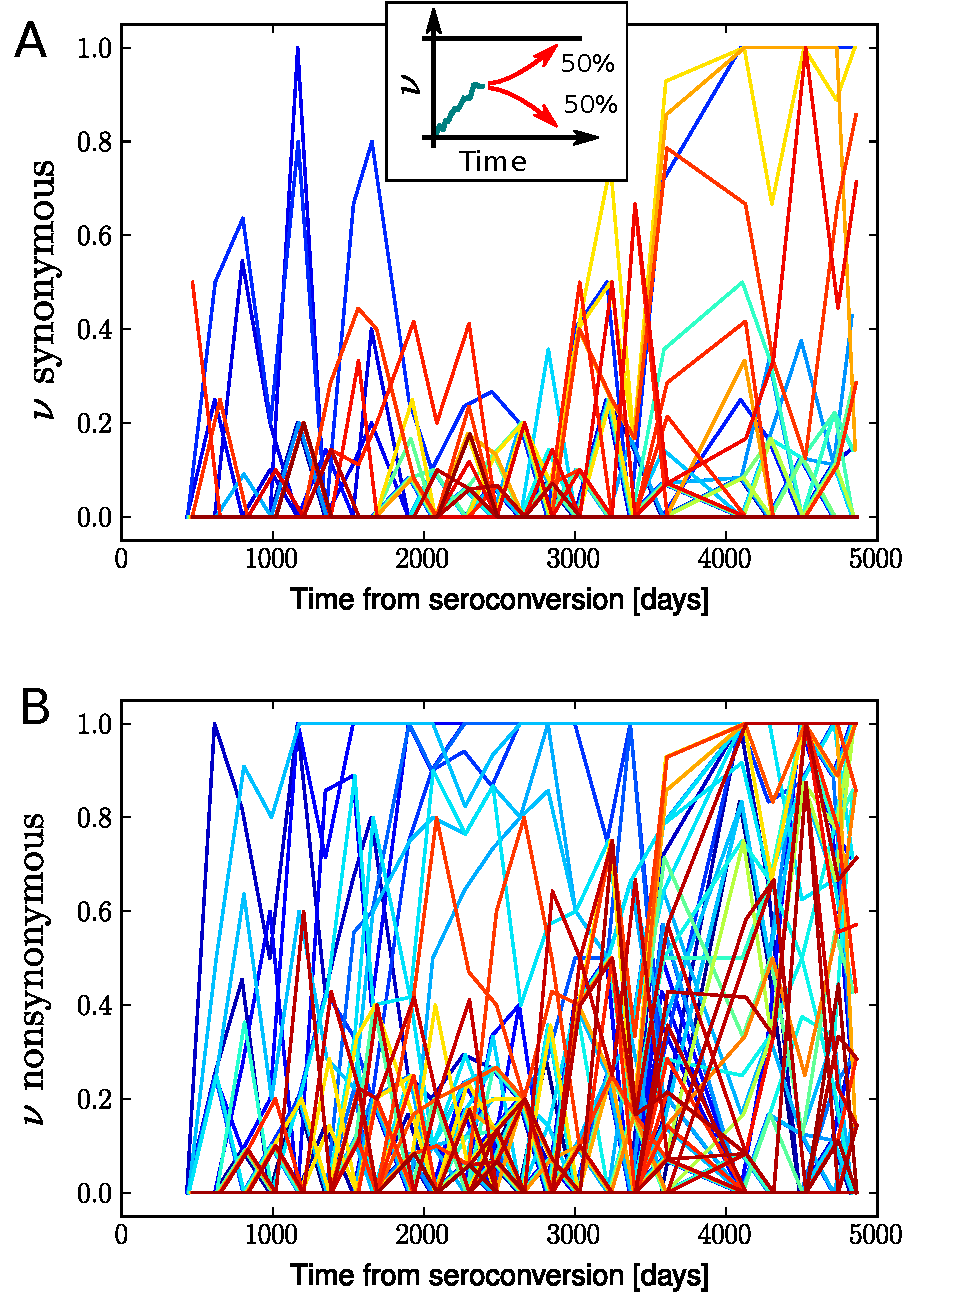
\includegraphics[width=0.6\linewidth]{fig1}
\caption{Time series of frequencies
of synonymous (A) and nonsynonymous (B) single nucleotide variants (SNVs) in \env, 
\shankaregion, from patient p10~\cite{shankarappa_consistent_1999}.
While many nonsynonymous SNVs fix, few synonymous
SNVs do so even though they are frequently observed at high
frequencies. Colors indicate the position of the site along the \shankaregion{} region
(blue to red). Inset: the fixation probability $\pfix$ of a neutral
SNV that reached 50\% frequency is one half.}
\label{fig:aft}
\end{center}
\end{figure}


\begin{figure}
\begin{center}
%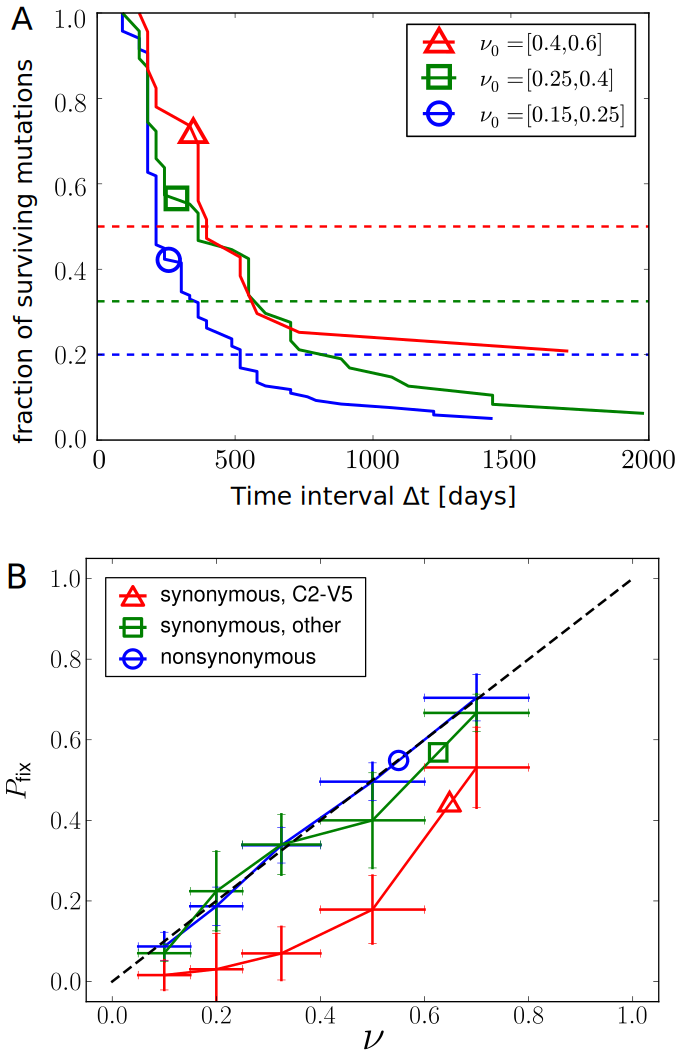
\includegraphics[width=0.6\linewidth]{fig2}
\caption{Fixation and loss of SNVs.
Panel A) shows how quickly synonymous SNVs are purged from the populations. 
Specifically, the figure shows the fraction of SNVs that are still observed
after $\Delta t$ days, conditional on being observed in one of the three frequency 
intervals (different colors). 
In each frequency interval, the fraction of synonymous
SNVs that ultimately survive is the fixation probability $\pfix$ conditional on the
initial frequency. The neutral expectation for $\pfix=\nu_0$ is indicated by 
dashed horizontal lines.
Panel B) shows the fixation probability of synonymous SNVs as a function of $\nu_0$. Polymorphisms within \shankaregion{} fix less
often than expected for neutral SNVs (indicated by the diagonal line).
This suppression is not observed in other parts of \env{} or for nonsynonymous
SNVs.
The horizontal error bars on the abscissa are bin sizes, the vertical ones the
standard deviation after 100 patient bootstraps of the data. Data from
refs.~\cite{shankarappa_consistent_1999,liu_selection_2006, bunnik_autologous_2008}.}
\label{fig:fixp}
\end{center}
\end{figure}

\begin{figure}
\begin{center}
%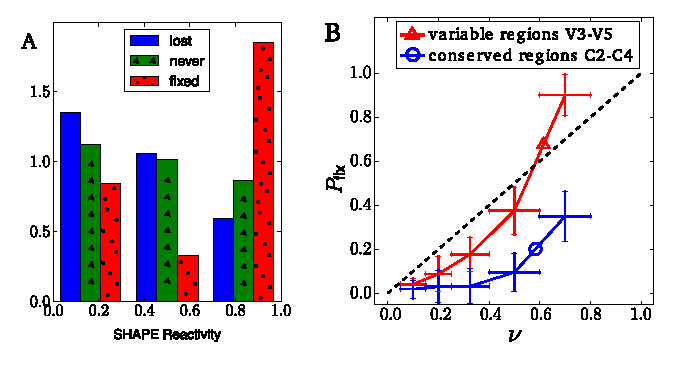
\includegraphics[width=0.9\linewidth]{fig3}
\caption{Permissible synonymous mutations tend to be unpaired.
Panel A) shows the distribution of SHAPE reactivities among sites at which synonymous 
SNVs fixed (red), sites at which SNVs reached frequencies above 15\% but
were subsequently lost (blue), and sites at which no high-frequency SNVs were observed (green) 
(all categories are restricted to the regions V1-V5$\pm 100$bp).
Sites at which SNVs fixed tend to have higher SHAPE reactivities, corresponding to
less base pairing, than those at which SNVs are lost.
Sites at which no SNVs are observed show an intermediate distribution of SHAPE values.
Panel B) shows the fixation probability of synonymous SNVs in
\shankaregion{} separately for variable regions V3-V5 and the connecting conserved 
regions C2-C4 that harbor RNA stems. As expected, the fixation probability is lower
inside the conserved regions. Data from Refs.~\cite{shankarappa_consistent_1999,
bunnik_autologous_2008, liu_selection_2006}.}
\label{fig:SHAPE}
\end{center}
\end{figure}

\begin{figure}
\begin{center}
%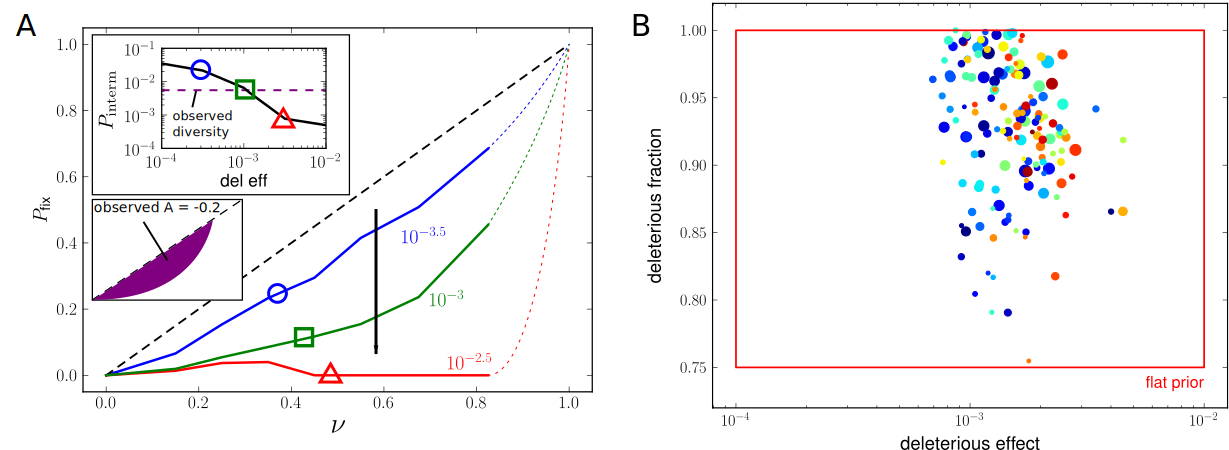
\includegraphics[width=0.6\linewidth]{fig4}
\caption{Distribution of selection coefficients on synonymous sites. Panel A)
The depression in $\pfix$ depends on the deleterious effect size 
of synonymous SNVs. This parameter also reduces synonymous
diversity, measured by the probability of a SNV to be found at
intermediate frequencies $P_\mathrm{interm}$ (first inset). The area observed in
the data is also shown (second inset).
Panel B) To assess the parameter space that affects synonymous fixation and
diversity, we run 3000 simulations with random combinations of parameters for deleterious effect
size, fraction of deleterious synonymous sites, average escape rate $\epsilon$,
rate of introduction of new epitopes, population size, mutation rate, and
recombination rate (see methods). The density of simulations that reproduce
the synonymous diversity and fixation patterns observed in data are shown.
These simulations demonstrate that deleterious effects are around $0.002$
and a large fraction of the synonymous mutations needs to be
deleterious. The marginal distributions of each parameter are given in
Fig.~S\marginals.} 
\label{fig:simheat}
\end{center}
\end{figure}

%%%%%%%%%%%%%%%%%%%%%%%%%%%%%%%%%%%%%%%%%%%%%%%%%%%%%%%%%%%%%%%%%%%%%%%%%
\end{document}
%%%%%%%%%%%%%%%%%%%%%%%%%%%%%%%%%%%%%%%%%%%%%%%%%%%%%%%%%%%%%%%%%%%%%%%%%
